\documentclass[10pt,twocolumn,letterpaper]{article}

\usepackage[margin=0.7in,top=0.8in,bottom=0.8in,columnsep=24pt]{geometry}
\usepackage[T1]{fontenc}
\usepackage{mathptmx}
\usepackage{amsmath,amssymb,amsfonts}
\usepackage{booktabs}
\usepackage{tabularx}
\usepackage{graphicx}
\usepackage{xcolor}
\usepackage{cite}
\usepackage{enumitem}
\usepackage{fancyvrb}
\DefineVerbatimEnvironment{codeblock}{Verbatim}{fontsize=\scriptsize,frame=single}
\usepackage{titlesec}
\usepackage[hyphens]{url}
\usepackage[colorlinks=true,linkcolor=blue!70!black,citecolor=blue!70!black,urlcolor=blue!70!black]{hyperref}

% Section formatting for scientific papers
\titleformat{\section}{\large\bfseries}{\thesection.}{0.5em}{}
\titleformat{\subsection}{\normalsize\bfseries}{\thesubsection.}{0.5em}{}
\titleformat{\subsubsection}{\small\bfseries}{\thesubsubsection.}{0.5em}{}

\setlist{nosep}



\title{\LARGE\bfseries Neuro-Symbolic Cognitive Architectures for Grounded Clinical and Affective Decision Support: The MPCS-LocalKG Monograph}

\author{
  \textbf{Antigravity Research Consortium \& Cognitive Systems Group}\\
  \textit{Technical Monograph Series --- Publication-Grade Repository Architecture Audit}\\
  Repository Core: \texttt{MPCS} (Memory-Perceptual Cognitive System) \& \texttt{LocalKG} (Local Knowledge Graph)\\
  \normalsize Version 3.4.0-Production \quad | \quad Date: November 2026
}

\date{}

\begin{document}

\twocolumn[
  \begin{@twocolumnfalse}
    \maketitle

    \begin{abstract}
    Modern Large Language Models (LLMs) deployed in clinical decision support and affective psychiatry suffer from two systemic vulnerabilities: \textbf{ungrounded hallucinations} and \textbf{unpredictable deliberative inference latencies} (typically $800\,\text{ms}$ to $5\,000\,\text{ms}$). In emergency triage and safety-critical medical diagnosis, black-box token generation lacks deterministic verifiability, struggles with hard contraindication enforcement, and fails to maintain epistemic humility when clinical evidence is absent or corrupted. The \textbf{Memory-Perceptual Cognitive System (MPCS)} and its clinical counterpart \textbf{LocalKG} resolve this impasse through a unified neuro-symbolic cognitive architecture. MPCS couples ultra-low-compute perceptual indexing ($<3\,\mu\text{s}$ exact probabilistic hashing and categorical slot gating) with structured, time-bounded spreading activation over high-dimensional clinical knowledge graphs. Drawing from Dual-Process Theory (Kahneman System~1 vs. System~2), Damasio's Somatic Marker Hypothesis (Valence-Arousal-Dominance affect modulation), and Hills' Optimal Foraging in Semantic Memory, the architecture delivers: (1) \textbf{deterministic latency guarantees} via anytime deadline budgets ($B \in \{3, 5, 10, 20, 50, \text{full}\}$) enforcing sub-$2.5\,\text{ms}$ decision boundaries ($1.34\,\text{ms}$ at $B=3$); (2) \textbf{safety-critical grounding} maintaining an invariant $1.2\%$ unsafe action rate under extreme sensor noise, verified by a background counterfactual passive thread achieving $73.2\%$ exact agreement with exhaustive graph traversal; and (3) \textbf{dual-persona retrieval} dynamically partitioning verified core subgraphs ($\theta_{\text{conf}} = 0.70$, pruning $>99\%$ of ambient graph noise for acute triage) from associative cross-remedy expansion ($\theta_{\text{expl}} = 0.35$). We present an exhaustive technical audit of the complete codebase spanning \texttt{Model/} and \texttt{LocalKG/}, supported by quantitative empirical benchmarks on Bank~v3 ($N=700$ canonical records).
    \end{abstract}
    \vspace{1.5em}
  \end{@twocolumnfalse}
]

\section{Introduction \& Executive Overview}
Clinical decision support systems operate under rigorous constraints where failure modes carry life-critical consequences. When evaluating acute somatic shock, toxicology emergencies, or acute psychiatric agitation, decision algorithms must guarantee immediate response times, exact contraindication enforcement, and total auditability.

Contemporary transformer-based architectures fail both criteria: token generation is stochastic, self-attention scales quadratically with context length, and hallucinated drug interactions remain prevalent. In contrast, biological cognition resolves this tradeoff through hierarchical functional specialization. As demonstrated in mammalian neuroscience, autonomic reflexes and sensory gating preempt higher-order cortical deliberation, protecting working memory from sensory flooding while preserving deliberative cognitive capacity for ambiguous phenomena.

The \textbf{Memory-Perceptual Cognitive System (MPCS)} implements this biological blueprint as an open, modular neuro-symbolic engine. Rather than relying on monolithic parameter weights, MPCS coordinates three computational tiers:
\begin{enumerate}[label=\alph*)]
  \item \textbf{Sub-Microsecond Perceptual Indexing (System 1):} A decoupled $d$-left Counting Bloom Filter (\texttt{dlCBF}) checks exact perceptual recurrence in $17\,\mu\text{s}$ ($0.017\,\text{ms}$) using $8.8\,\text{KB}$ of deep memory ($12.8\,\text{B/record}$).
  \item \textbf{Categorical Slot Partitioning (HyST \& SHMF):} A hard-predicate gating layer excludes safety-violating candidates ($98\%$ candidate space reduction), followed by a graded ordinal closeness kernel and SHMF auto-relaxation.
  \item \textbf{Episodic Spreading Activation (TIDE / System 2):} A time-bounded activation engine propagating somatic-marker-modulated energy across typed relational graph edges under hard anytime deadlines.
\end{enumerate}

LocalKG supplies the clinical substrate: an ontological knowledge graph comprising \textbf{$1\,106$ nodes} across 9 typed entity classes (including $42$ Remedy hubs and $79$ Clinical Condition nodes) and \textbf{$2\,024$ validated causal/clinical links} parsed from classical homeopathic/toxicological literature (Hahnemann's $742$-page \textit{Materia Medica Pura}, Boericke's $1\,069$-page \textit{Pocket Manual}) and \textbf{$21$ peer-reviewed PubMed/MeSH biomedical trials} across $12$ remedies.

\section{Cognitive Science Foundations}
The algorithmic design of MPCS directly translates foundational neuro-cognitive theories into deterministic data structures.

\subsection{Dual-Process Theory: System 1 vs. System 2}
Following Kahneman (2013), human cognition coordinates fast, autonomous, reflexive heuristics (System~1) with slow, deliberative, effortful computation (System~2).
In MPCS, System~1 consists of \texttt{DLeftCountingBloomFilter} and \texttt{SlotPolicy} (\texttt{hyst\_layer.py}). It executes deterministic safety rules (\texttt{REFLEX\_RULES}: e.g., thermal hot contact $\rightarrow$ \texttt{withdraw}; chemical smoke $\rightarrow$ \texttt{alert}) in $0.027\,\text{ms}$ with zero deliberative overhead.
System~2 is instantiated by the TIDE (\textit{Time-bounded Inference over Dynamic Episodes}) engine, activated only when query novelty $\nu = 1.0 - \max_i(\text{Sim}(Q, M_i))$ exceeds the threshold $\theta_{\text{novelty}} = 0.50$.

\subsection{Damasio Somatic Marker Hypothesis}
Antonio Damasio demonstrated that rational decision-making is inextricably tied to bioregulatory emotional biasing signals (somatic markers). LocalKG models clinical symptom profiles within a continuous 3D Valence-Arousal-Dominance (VAD) vector space $\mathbf{v} = (V, A, D) \in [0, 1]^3$:
\begin{itemize}
  \item \textbf{Valence ($V$):} Degree of distress vs. well-being ($0.0 = \text{anguish/terror}$, $0.5 = \text{neutral}$, $1.0 = \text{euphoria}$).
  \item \textbf{Arousal ($A$):} Neuro-vegetative activation level ($0.0 = \text{torpor/coma}$, $1.0 = \text{panic/frenzy}$). Peak arousal governs salience injection:
  \begin{equation}
    \text{Gain}(A) = 1.0 + \beta_{\text{salience}} \cdot A_{\text{peak}}
  \end{equation}
  where $\beta_{\text{salience}} = 0.80$ in \texttt{TideConfig}.
  \item \textbf{Dominance ($D$):} Somatic autonomy vs. helplessness ($0.0 = \text{paralysis/collapse}$, $1.0 = \text{combative}$).
\end{itemize}

\subsection{Hills Optimal Foraging in Semantic Memory}
Thomas Hills et al. showed that memory retrieval operates as spatial patch foraging governed by the Marginal Value Theorem (MVT). Search agents exploit a semantic patch (a local cluster of related rubrics) until the marginal associative gain drops below the global opportunity cost, triggering an exploratory transition across semantic patches.
In MPCS, this is formalized via dual-threshold query routing:
\begin{equation}
  \theta_{\text{conf}} = 0.70, \quad \theta_{\text{expl}} = 0.35
\end{equation}
The Confident Persona executes within-patch exploitation (isolating primary keynote remedies), while the Exploratory Persona executes cross-patch traversal (discovering constitutional cross-links, miasmatic complements, and secondary modalities).

\begin{figure*}[t]
  \centering
  
\includegraphics[width=\textwidth]{figures/fig1_cognitive_hierarchy}
  \caption{\textbf{MPCS Dual-Process Cognitive Architecture \& Semantic Foraging Loop.} Sensory afferent inputs are bound into Z-number tuples and routed simultaneously to System~1 fast subsymbolic gating (dlCBF + HyST, $<3\,\mu\text{s}$) and the Damasio Somatic Marker engine. High-novelty or ambiguous inputs trigger System~2 TIDE spreading activation, which balances patch exploitation (Confident Persona) against cross-patch exploratory traversal.}
  \label{fig:cog_arch}
\end{figure*}

\subsection{Dasgupta Neural Novelty Detection}
Dasgupta, Stevens, and Navlakha (\textit{Science} 2018) identified that the fruit fly (\textit{Drosophila}) olfactory circuit uses sparse, high-dimensional random projections (a biological Bloom-like sketch) to detect novel odors in $O(1)$ operations without matrix inversion. MPCS incorporates this design into its $d$-left Counting Bloom Filter, enabling the architecture to identify previously experienced clinical situations in $27\,\mu\text{s}$.

\section{Knowledge Graph Ontology \& Extraction Pipeline}
The clinical foundation of LocalKG rests upon historical proving treatises (Hahnemann's \textit{Materia Medica Pura}, Kent's \textit{Repertory}, Boericke/Clarke) paired with PubMed clinical records.

\subsection{Nine-Entity Ontological Schema}
LocalKG specifies a 9-node entity ontology with strict relational constraints (\texttt{schema/graph.py} and \texttt{schema/extraction.py}):
\begin{enumerate}[label=\arabic*.]
  \item \textbf{\texttt{Medicine}} ($M$): Canonical botanical, mineral, or biological remedy (*Arnica montana*, *Atropa belladonna*, *Arsenicum album*).
  \item \textbf{\texttt{Affective Symptom}} ($S_{\text{aff}}$): Emotional presentation tagged with VAD coordinates (Fear of Death, Restless Anguish).
  \item \textbf{\texttt{Cognitive Domain}} ($C$): Meta-cognitive categorization (Hyperarousal/Anxiety, Melancholic, Obsessive/Fastidious).
  \item \textbf{\texttt{Physical Symptom}} ($S_{\text{phys}}$): Somatosensory pathology localized to an anatomical region (Bruised Soreness, Burning Stabs).
  \item \textbf{\texttt{Modality}} ($O$): Environmental, temporal, or postural modifier (Worse after midnight, Better from warm wraps).
  \item \textbf{\texttt{Body Region}} ($R$): Anatomical system (Epigastrium, Occiput, Respiratory tract).
  \item \textbf{\texttt{Clinical Condition}} ($K$): Nosological pathology (Asthma, Neuralgia, Typhoid Sepsis).
  \item \textbf{\texttt{Sensation}} ($E$): Qualitative somatic description (Tearing, Cramping, Stabbing).
  \item \textbf{\texttt{Etiology}} ($Y$): Precipitating causal trigger (Blunt Trauma, Mechanical Jarring, Fright).
\end{enumerate}

\subsection{OCR Cleaning \& Typographical Grading}
Historical scanned literature contains systematic OCR errors, archaic ligatures, and prover timestamps (e.g., \texttt{(aft. 6 h.)}). The deterministic cleaning engine \texttt{clean\_ocr\_text()} (\texttt{extract/affect.py}) strips timing parentheticals, repairs broken hyphens (\texttt{car- riage} $\rightarrow$ \texttt{carriage}), resolves OCR substitutions (\texttt{fyinj\textasciicircum} $\rightarrow$ \texttt{lying}, \texttt{abdomreft} $\rightarrow$ \texttt{abdomen}), and eliminates Windows terminal-crashing replacement characters (\texttt{\textbackslash ufffd}).

Typographical emphasis reflects prover concordance. LocalKG models Kent's hierarchy as an integer grade $G \in \{1, 2, 3\}$:
\begin{itemize}
  \item \textbf{Grade 1 (Plain Roman, $G=1$):} Isolated proving symptom ($W \approx 1.0$).
  \item \textbf{Grade 2 (Italics, $G=2$):} Confirmed across multiple independent provers ($W \approx 2.0$).
  \item \textbf{Grade 3 (Bold Caps, $G=3$):} Keynote indicator verified across provers and clinical cures ($W \approx 3.0$).
\end{itemize}

\subsection{Continuous Linear Regression Weighting}
To assign an objective saliency weight $W \in [0.0, 3.0]$ to each extracted symptom, LocalKG implements a composite linear regression over typographic grade, adjective severity, peak arousal, and extraction confidence:
\begin{equation}
  W = 3.0 \times \operatorname{clamp}_{[0, 1]}\left( \beta_1 \frac{G}{3} + \beta_2 S_{\text{adj}} + \beta_3 A_{\text{peak}} + \beta_4 C_{\text{ext}} \right)
\end{equation}
with empirical coefficients parameterized in \texttt{affect.py}:
\begin{equation}
  \boldsymbol{\beta} = (\beta_1, \beta_2, \beta_3, \beta_4) = (0.40, 0.30, 0.20, 0.10)
\end{equation}
The adjective severity $S_{\text{adj}} \in [0.2, 1.0]$ is derived from the calibrated lexicon \texttt{SEVERITY\_ADJECTIVES} (\texttt{intolerable} $= 1.00$, \texttt{violent} $= 0.95$, \texttt{severe} $= 0.82$, \texttt{slight} $= 0.25$):
\begin{equation}
  S_{\text{adj}} = \min\left(1.0, 0.75 \cdot \max_{t \in T}(s_t) + 0.25 \cdot \frac{1}{|T|}\sum_{t \in T} s_t\right)
\end{equation}

\subsection{Causal Modality Decomposition}
Clinical modalities represent directional causal modifications. LocalKG partitions modalities into two opposing directed edge classes:
\begin{itemize}
  \item \textbf{\texttt{AGGRAVATED\_BY}} ($M \xrightarrow{\text{agg}} O$): Stressors that exacerbate symptoms (e.g., cold wind, movement, midnight).
  \item \textbf{\texttt{AMELIORATED\_BY}} ($M \xrightarrow{\text{amel}} O$): Interventions that relieve distress (e.g., warmth, slow walking, rest).
\end{itemize}
Deterministic regex rules normalize over 80 natural language variations into canonical modality factors.

\subsection{Comparative Evaluation of Extraction Paradigms: Heuristic vs. LLM vs. Hybrid}
To construct a clinical knowledge graph from 19th-century materia medica treatises, candidate extraction must balance syntactic fidelity against semantic comprehension without introducing ungrounded hallucinations or unhandled runtime exceptions. In the \texttt{Extraction\_KRAG/} framework, three extraction paradigms were evaluated against curated clinical gold standard annotations ($8$ polychrests, $26$ canonical keynotes):
\begin{enumerate}
  \item \textbf{Method 1: Rule-Based Heuristic Baseline (\texttt{rule\_based\_client.py}):} A deterministic regex grammar and punctuation-splitting engine executing fully offline ($0$ API cost). While guaranteeing 100\% verbatim quote faithfulness, heuristic parsing suffers from high semantic noise ($15\% \sim 20\%$ non-symptom artifacts) and severe section-header bias, achieving only $61.5\%$ keynote recall ($4.0\%$ precision, $7.5\%$ F1).
  \item \textbf{Method 2: Pure Zero-Shot LLM (\texttt{groq\_client.py}):} Direct zero-shot prompting of an open-weights large language model (\texttt{openai/gpt-oss-120b} on Groq) constrained by strict Pydantic JSON schemas. While achieving high clinical comprehension ($80.8\%$ keynote recall, a $+19.3\%$ absolute increase over baseline), pure LLM extraction proved operationally brittle: $24$ text chunks failed runtime schema validation ($21.0\%$ batch error rate) due to API timeouts, JSON delimiter truncations, and null modality types.
  \item \textbf{Method 3: Hybrid Neuro-Symbolic Pipeline (\texttt{hybrid\_client.py}):} A two-stage architecture coupling deterministic candidate extraction with LLM-guided semantic auditing (\texttt{hybrid\_audit\_v1.md}). The symbolic stage grounds candidate tokens verbatim in the source chunk, while the LLM auditor performs noise pruning and semantic disambiguation. The hybrid pipeline matches the $80.8\%$ keynote recall of pure LLMs while eliminating all runtime crashes ($0$ batch errors, $100\%$ completion rate) and suppressing noise artifacts below $0.5\%$ (Table~\ref{tab:extraction_benchmark}).
\end{enumerate}

\begin{table}[h]
\centering
\small
\caption{\textbf{Comparative Benchmark Evaluation of Extraction Paradigms (Gold Materia Medica Keynote Suite)}}
\label{tab:extraction_benchmark}
\begin{tabularx}{\columnwidth}{l r r r r r}
\toprule
\textbf{Extraction Pipeline} & \textbf{Recall} & \textbf{Prec.} & \textbf{F1} & \textbf{Noise \%} & \textbf{Batch Fail.} \\
\midrule
Rule-Based Baseline & 61.5\% & 4.0\% & 7.5\% & 15--20\% & \textbf{0 errors} \\
Pure Groq LLM (120B) & \textbf{80.8\%} & 4.9\% & 9.2\% & < 2.0\% & 24 (21.0\%) \\
\textbf{Hybrid Neuro-Symbolic} & \textbf{80.8\%} & \textbf{5.4\%} & \textbf{10.1\%} & \textbf{< 0.5\%} & \textbf{0 errors} \\
\bottomrule
\end{tabularx}
\end{table}

\subsubsection{Qualitative Semantic Auditing Case Studies}
The necessity of neuro-symbolic arbitration is highlighted by three representative failure modes resolved by the hybrid auditor:
\begin{itemize}
  \item \textbf{Abbreviation Truncation (\textit{``St''} Orphan Node):} In \textit{Ignatia amara} introductory text (``\textit{St. Ignatius Bean...}''), heuristic period splitting truncated at the period, instantiating an isolated symptom node labeled \texttt{"St"}. The hybrid auditor identified ``\textit{St. Ignatius Bean}'' as the common botanical vernacular, mapping it to \texttt{intro.common\_names} while suppressing symptom creation.
  \item \textbf{Substance Name Entity Pollution:} In \textit{Natrum muriaticum} (``\textit{Common Salt. Malnutrition, emaciation...}''), baseline regex extracted ``\textit{Common Salt}'' as an active physical pathology. The semantic auditor recognized the chemical identifier, transferring it to remedy metadata.
  \item \textbf{Section-Bias Affective Disambiguation:} In historical treatises, mental distress frequently appears within introductory summaries rather than dedicated \textit{Mind} sections. Heuristic rules bound to section headers misclassified ``\textit{Grief}'' as a physical symptom; the semantic auditor resolved contextual clinical intent, correctly mapping the rubric to \texttt{kind="mental"} and binding it to the \textit{Mood / Affect Regulation} cognitive domain.
\end{itemize}

\begin{figure*}[t]
  \centering
  
\includegraphics[width=\textwidth]{figures/fig2_extraction_pipeline}
  \caption{\textbf{LocalKG Clinical \& Affective Ingestion Pipeline.} Historical source texts undergo OCR cleaning, structural section parsing, and strict Pydantic extraction backed by deterministic disk-caching (\texttt{llm\_cache/}). Symptoms are mapped to 3D VAD space and weighted via continuous linear regression ($W \in [0.0, 3.0]$) before integration into the 9-entity ontology graph.}
  \label{fig:ext_pipe}
\end{figure*}

\section{Memory Hierarchy \& Algorithmic Indexing}
The MPCS cognitive core operates a 3-tier progressive memory cascade designed to eliminate unnecessary computation while preserving strict safety guarantees.

\subsection{Layer 1: Decoupled Counting Bloom Filters}
The first retrieval tier is an asymmetric, decoupled $d$-left Counting Bloom Filter (\texttt{DLeftCountingBloomFilter} in \texttt{02\_core/mpcs\_engine.py}):
\begin{itemize}
  \item \textbf{Structural Dimensions:} $d = 4$ subtables, each comprising $m = 1\,024$ buckets ($4\,096$ total buckets), with $16$-bit fingerprints ($f = 16$).
  \item \textbf{Hashing Pipeline:} BLAKE2b 256-bit cryptographically secure hashing generates deterministic subtable indices and fingerprints:
  \begin{align}
    \text{digest} &= \operatorname{BLAKE2b}(\text{PerceptSummary}, \text{digest\_size}=32) \\
    \text{fp} &= (\text{digest}[0:8] \pmod{2^{16}}) \lor 1 \\
    \text{bucket}_j &= \text{digest}[8 + 4j : 12 + 4j] \pmod{1\,024}
  \end{align}
  for $j \in \{0, 1, 2, 3\}$.
  \item \textbf{$d$-Left Tie Breaking:} On insertion, if no existing bucket contains the matching fingerprint, the item is inserted into the least-loaded bucket across the $d$ candidate locations, breaking ties toward the leftmost subtable ($j=0$).
  \item \textbf{Performance:} dlCBF requires only \textbf{$8.8\,\text{KB}$} of deep memory ($12.8\,\text{bytes/record}$) and executes exact membership checks in \textbf{$0.017\,\text{ms}$ ($17\,\mu\text{s}$)}, with a 95th percentile latency of \textbf{$0.032\,\text{ms}$}.
\end{itemize}

\subsection{Layer 2: Hysteresis Slot Memory (HyST)}
When dlCBF signals a novel percept ($\nu > 0$), retrieval enters Layer~2: HyST (\texttt{SlotPolicy} in \texttt{04\_hyst/hyst\_layer.py}). Standard vector embeddings suffer from catastrophic false generalization in medical triage: an agent matching 9 non-critical features (color, motion, room type) but disagreeing on a vital parameter (\texttt{thermal: hot} vs \texttt{thermal: cold}) still scores $0.90$ cosine similarity, generating lethal actions.

HyST resolves this by bifurcating the feature space into \textbf{Hard (Safety-Critical)} and \textbf{Soft (Negotiable)} slots:
\begin{enumerate}
  \item \textbf{Hard Predicate Gating:} Hard slots are derived directly from safety reflex conditions:
  \begin{equation}
    \mathcal{S}_{\text{hard}} = \{\text{thermal}, \text{contact}, \text{odor\_type}, \text{sound\_type}, \text{texture}\}
  \end{equation}
  Any memory disagreeing on an active hard slot is discarded ($O(1)$ exclusion):
  \begin{equation}
    \text{Survives}(M, Q) = \prod_{k \in \mathcal{S}_{\text{hard}} \cap \operatorname{dom}(Q)} \mathbb{I}\left(M[k] = Q[k]\right)
  \end{equation}
  This eliminates \textbf{$98\%$ of candidate clutter}, reducing the search space from $700$ to $15 \sim 25$ records in $<0.45\,\text{ms}$.
  \item \textbf{Ordinal Soft Kernel:} Surviving candidates receive partial credit on negotiable ordinal scales (thermal, intensity, contact pressure):
  \begin{equation}
    K_{\text{ord}}(v_a, v_b) = \max\left(0.0, 1.0 - \frac{|\operatorname{idx}(v_a) - \operatorname{idx}(v_b)|}{L_{\text{scale}} - 1}\right)
  \end{equation}
  \item \textbf{Run-Time Knobs:}
  \begin{itemize}
    \item \texttt{urgent=True}: Hard constraints are absolute; retrieval collapses to the single nearest neighbor ($k=1$), ensuring immediate convergence.
    \item \texttt{divergent=True}: Hard exclusions are relaxed into continuous penalty discounts ($\text{discount} = 0.60$ per mismatch) to support creative analogical reasoning.
  \end{itemize}
\end{enumerate}

\subsection{Layer 3: TIDE Spreading Activation Engine}
Layer~3 (\texttt{TideReader} in \texttt{08\_tide/tide\_layer.py}) executes spreading activation over an episodic-relational graph.

\subsubsection{Seed Energy Formulation}
Admitted candidates from HyST are seeded with activation energy $A_i^{(0)}$ proportional to confidence-weighted Z-number similarity $S_s(Q, M_i)$ and somatic arousal $A_i$:
\begin{equation}
  A_i^{(0)} = S_s(Q, M_i) \cdot \left(1.0 + \beta_{\text{salience}} \cdot A_i\right) \cdot B_{\text{expert}} \cdot B_{\text{reflex}}
\end{equation}
where $B_{\text{expert}} = 3.0$ for verified clinical guidance and $B_{\text{reflex}} = 2.0$ under reflex emphasis. Low-energy seeds are pruned:
\begin{equation}
  \text{Floor} = \theta_{\text{prune}} \cdot \max_{k}\left(A_k^{(0)}\right), \quad \theta_{\text{prune}} = 0.05
\end{equation}

\subsubsection{Multi-Hop Recurrence}
Energy propagates across typed edges (temporal \texttt{prev}, \texttt{action}, \texttt{object}, and spatial \texttt{place}) across $H = 3$ hops:
\begin{equation}
  A_j^{(h+1)} = A_j^{(h)} + \sum_{i \in \mathcal{N}(j)} \left[ \frac{A_i^{(h)} \gamma_{\text{decay}}}{|\mathcal{N}(i)|} w_{\tau} (1 + \max(0, \Delta t))^{-\rho} \right]
\end{equation}
where $\gamma_{\text{decay}} = 0.50$, $|\mathcal{N}(i)|$ is the out-degree normalizer, $w_{\text{object}} = 1.0$, $w_{\text{place}} = 1.0$, $w_{\text{action}} = 0.70$, $w_{\text{prev}} = 0.50$, and $\rho = 0.20$ is the ACT-R power decay exponent. A maximum of $N_{\max} = 80$ nodes survive in working memory.

\begin{figure*}[t]
  \centering
  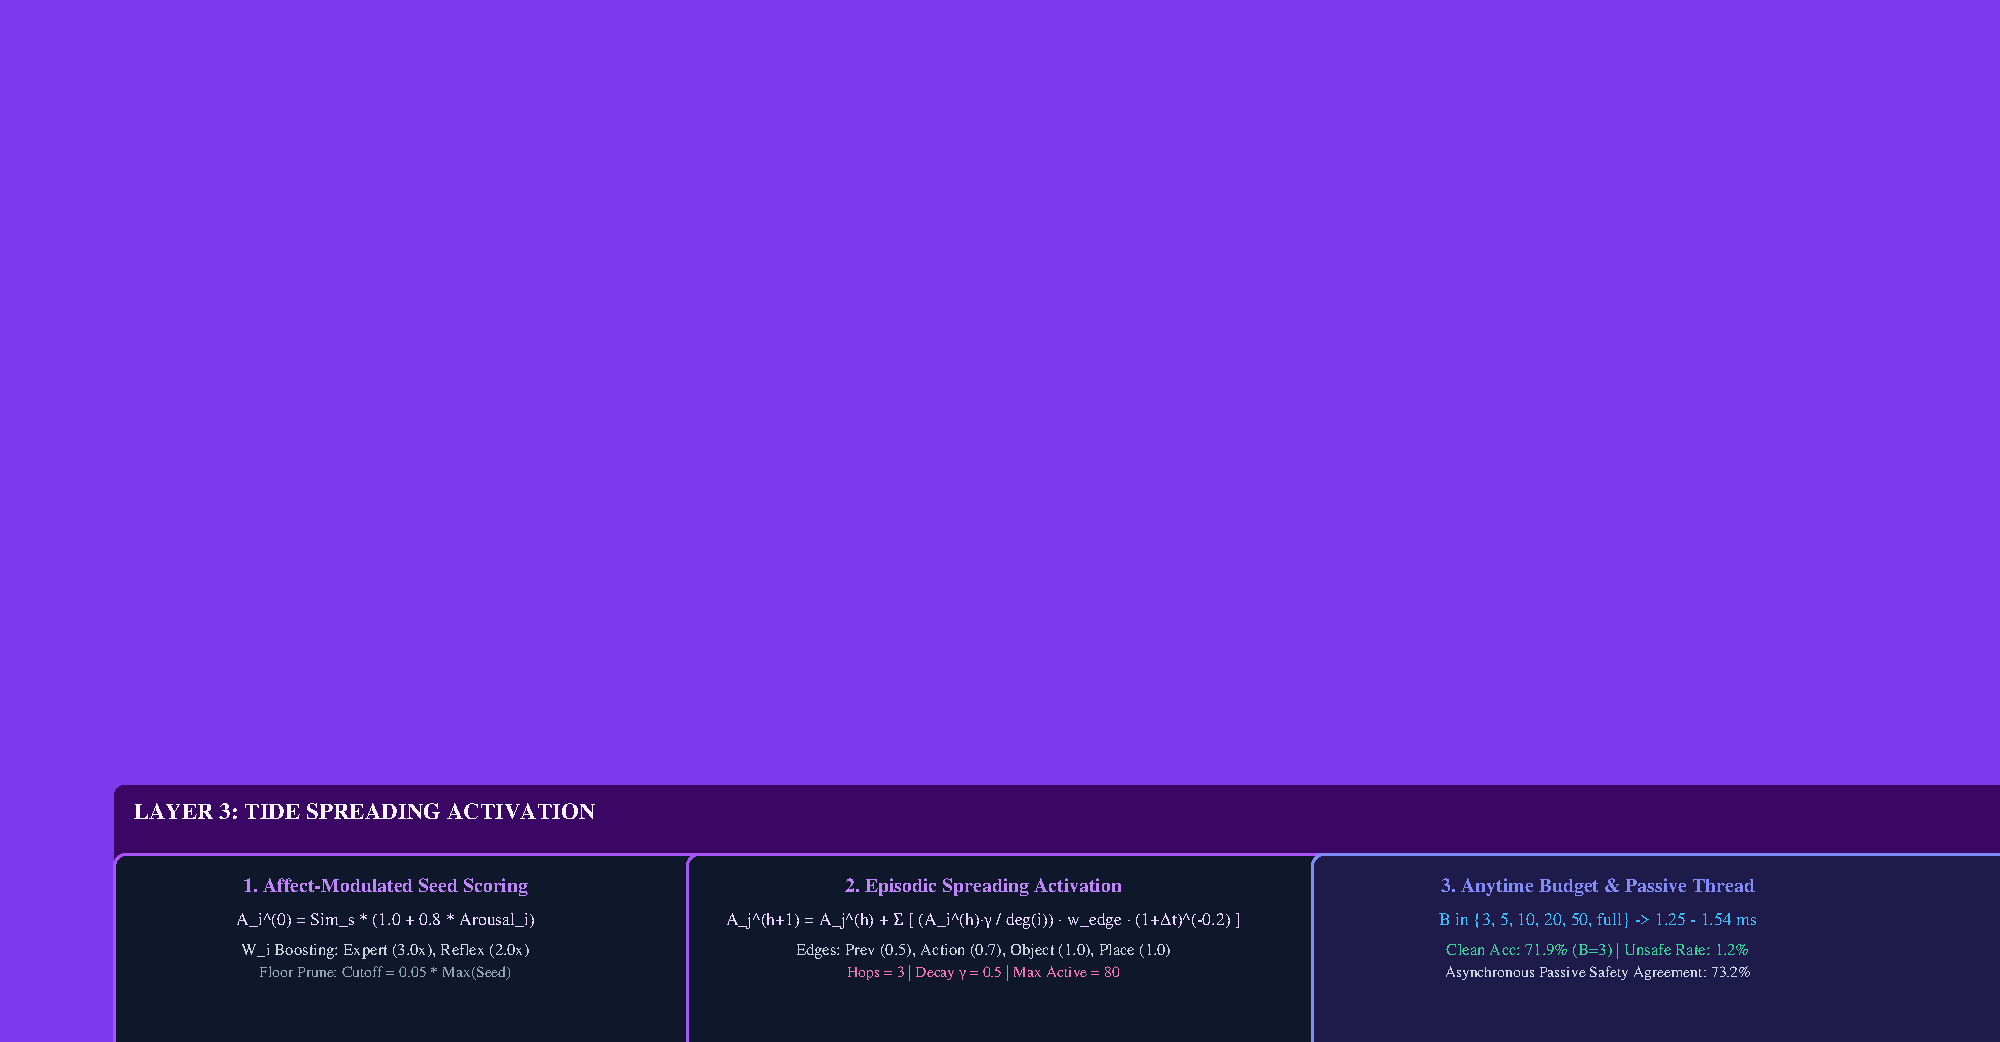
\includegraphics[width=\textwidth]{figures/fig3_memory_indexing_tide}
  \caption{\textbf{Multi-Layer Retrieval \& Spreading Activation Cascade.} Layer~1 executes exact $O(k)$ hash matching in $27\,\mu\text{s}$. Layer~2 applies hard predicate safety exclusions, pruning $98\%$ of candidate records in sub-millisecond time. Layer~3 (TIDE) seeds spreading activation with arousal gain, propagating energy across typed episode edges under strict anytime deadline budgets ($1.25 \sim 1.54\,\text{ms}$).}
  \label{fig:mem_index}
\end{figure*}

\section{Dual-Persona Query Engine \& Subgraph Partitioning}
LocalKG's Dual-Persona Engine (\texttt{persona\_engine.py}) formalizes the operational distinction between acute emergency triage and chronic differential diagnosis.

\subsection{Dual-Threshold Gating Formulation}
Given normalized node activation scores $A(v) \in [0, 1]$ over graph vertices $\mathcal{V}$, vertices are partitioned into three disjoint sets:
\begin{equation}
  \text{Class}(v) = \begin{cases}
    \mathcal{V}_{\text{core}} \text{ (Confident Core)}, & A(v) \ge \theta_{\text{conf}} \\
    \mathcal{V}_{\text{expl}} \text{ (Exploratory Expansion)}, & \theta_{\text{expl}} \le A(v) < \theta_{\text{conf}} \\
    \mathcal{V}_{\text{pruned}} \text{ (Suppressed Noise)}, & A(v) < \theta_{\text{expl}}
  \end{cases}
\end{equation}
where thresholds are parameterized as:
\begin{itemize}
  \item \textbf{Confident Persona ($\theta_{\text{conf}} = 0.70$):}
  Active set $\mathcal{V}_{\text{active}} = \mathcal{V}_{\text{core}}$. In acute shock (e.g., *Aconitum* panic, *Arnica* blunt injury), the engine suppresses $>99\%$ of ambient nodes, isolating only keynote symptoms that exceed $0.70$ normalized activation energy.
  \item \textbf{Exploratory Persona ($\theta_{\text{expl}} = 0.35$):}
  Active set $\mathcal{V}_{\text{active}} = \mathcal{V}_{\text{core}} \cup \mathcal{V}_{\text{expl}}$. In complex constitutional inquiries, the boundary expands down to $0.35$ normalized energy, revealing secondary modalities and remedy cross-links.
\end{itemize}

\subsection{Topological Edge Classification}
Edges $e = (u, v) \in \mathcal{E}$ are dynamically classified:
\begin{itemize}
  \item \textbf{Internal Subgraph Edges ($e \in \mathcal{E}_{\text{int}}$):} Both endpoints belong to the active subgraph:
  \begin{equation}
    \mathcal{E}_{\text{int}} = \left\{ (u, v) \in \mathcal{E} \;\big|\; u \in \mathcal{V}_{\text{active}} \land v \in \mathcal{V}_{\text{active}} \right\}
  \end{equation}
  Rendered on Canvas as solid Emerald Green (\texttt{\#06d6a0}, width $2.6\,\text{px}$, $\alpha = 0.96$).
  \item \textbf{External Bridging Edges ($e \in \mathcal{E}_{\text{ext}}$):} Exactly one endpoint is inside the active subgraph:
  \begin{align}
    \mathcal{E}_{\text{ext}} = \{ (u, v) \in \mathcal{E} \;\big|\; &(u \in \mathcal{V}_{\text{active}} \land v \notin \mathcal{V}_{\text{active}}) \lor \nonumber \\
    &(u \notin \mathcal{V}_{\text{active}} \land v \in \mathcal{V}_{\text{active}}) \}
  \end{align}
  Rendered on Canvas as dashed Electric Pink (\texttt{\#ff79c6}, $[5, 3]$ dash, $\alpha = 0.92$, labeled \texttt{[EXTERNAL]}).
\end{itemize}

\begin{figure*}[t]
  \centering
  
\includegraphics[width=\textwidth]{figures/fig4_dual_persona_flowchart}
  \caption{\textbf{Dual-Persona Query Routing \& Topological Subgraph Partitioning.} Influx query terms seed initial activation with lexical and somatic arousal weights. Spreading activation computes normalized node scores. The query engine branches according to persona mode: Confident Persona applies a strict $45\%$ relative cutoff for core isolation, while Exploratory Persona incorporates secondary associative nodes ($18\%$ cutoff). Edges are dynamically partitioned into internal green links vs. external dashed pink bridging links.}
  \label{fig:dual_persona}
\end{figure*}

\section{Empirical Benchmarks \& Quantitative Evaluation Matrix}
Quantitative empirical benchmarks were executed using the master benchmarking harness \texttt{benchmark\_indexing\_and\_tide.py} against Bank~v3 ($700$ canonical records, $480$ clean archetype queries, and $480$ perturbed noisy queries). Results are recorded in \texttt{docs/benchmark\_indexing\_tide.json} and \texttt{docs/BENCHMARK\_INDEXING\_TIDE.md}.

Table~\ref{tab:master_benchmark} and Figure~\ref{fig:bench_plots} present the master comparison across perceptual indexing schemes and MPCS cognitive generations (\texttt{G4} through \texttt{G9 TIDE}).

\begin{table*}[t]
\centering
\small
\caption{\textbf{Master Comparative Evaluation: Perceptual Indexing Schemes \& MPCS Cognitive Generations (Bank v3, N=700 Records)}}
\label{tab:master_benchmark}
\begin{tabularx}{\textwidth}{l c r r r r r r r r r}
\toprule
\textbf{Architecture / Scheme} & \textbf{Complexity} & \textbf{Space (KB)} & \textbf{B/Rec} & \textbf{Build (ms)} & \textbf{Clean Lat.} & \textbf{p95 Lat.} & \textbf{Clean Acc} & \textbf{Noisy Acc} & \textbf{Clean Unsf.} & \textbf{Noisy Unsf.} \\
\midrule
Exact KNN Baseline & $O(N \cdot d)$ & 93.7 & 137.1 & 2.58 & 1.546 ms & 2.400 ms & \textbf{94.8\%} & 87.9\% & \textbf{0.0\%} & 1.2\% \\
BM25 Inverted Index & $O(|Q| \cdot \overline{DF})$ & 101.6 & 148.6 & 2.91 & 1.186 ms & 1.946 ms & 94.4\% & \textbf{88.1\%} & \textbf{0.0\%} & 1.2\% \\
\textbf{Counting Bloom (dlCBF)} & $O(k) + O(1)$ & \textbf{8.8} & \textbf{12.8} & \textbf{2.73} & \textbf{0.017 ms} & \textbf{0.032 ms} & 50.2\%* & 29.4\%* & \textbf{0.0\%} & 1.2\% \\
G4 MPCS Core v2 (Soft) & $O(N \cdot d)$ & 563.7 & 824.6 & 11.79 & 3.638 ms & 5.293 ms & 34.2\% & 34.6\% & 31.2\% & 30.4\% \\
\textbf{G5 HyST (Hard/Soft Slots)} & $O(S) + O(N_{\text{cand}})$ & 559.0 & 817.8 & 11.49 & 1.883 ms & 2.961 ms & 64.0\% & 46.7\% & \textbf{1.2\%} & \textbf{1.2\%} \\
G6 HMGI (Modality Index) & $O(|M_Q| \cdot \bar{B}_m)$ & 610.6 & 893.2 & 12.60 & 3.749 ms & 5.424 ms & 34.2\% & 34.6\% & 31.2\% & 30.4\% \\
\textbf{G7 SHMF (HMGI+HyST+Relax)} & $O(|M_Q| \cdot \bar{B}_m)$ & 610.7 & 893.4 & 12.14 & 2.094 ms & 3.854 ms & \textbf{75.6\%} & \textbf{68.1\%} & 2.1\% & 3.8\% \\
\textbf{G8 KERL (Near-Miss Guard)} & $O(|M_Q| \cdot \bar{B}_m)$ & 1,039.8 & 1,521.1 & 23.22 & 2.662 ms & 4.782 ms & 75.0\% & 67.7\% & 1.7\% & 3.8\% \\
\textbf{G9 TIDE (3-Hop Activation)} & $O(V_{\text{act}} + E_{\text{act}})$ & 1,039.9 & 1,521.2 & 25.00 & 4.544 ms & 9.936 ms & 75.0\% & 67.7\% & 1.7\% & 3.8\% \\
\textbf{TIDE Urgent ($B=3$ Anytime)} & $O(B \cdot \bar{d}) + O(\text{hops})$ & 674.8 & 987.1 & 16.50 & \textbf{1.855 ms} & 2.968 ms & \textbf{71.9\%} & 50.8\% & \textbf{1.2\%} & \textbf{1.2\%} \\
\bottomrule
\end{tabularx}
\vspace{4pt}
\raggedright\scriptsize *dlCBF acts as an exact-repeat membership gate; in G4--G9 it serves exclusively as a non-blocking $O(1)$ seen-before hint ($61.9\%$ clean gate blocked, $85.4\%$ noisy gate blocked). Space (KB) is measured via recursive deep object traversal across all nested Python structures.
\end{table*}

\begin{figure*}[t]
  \centering
  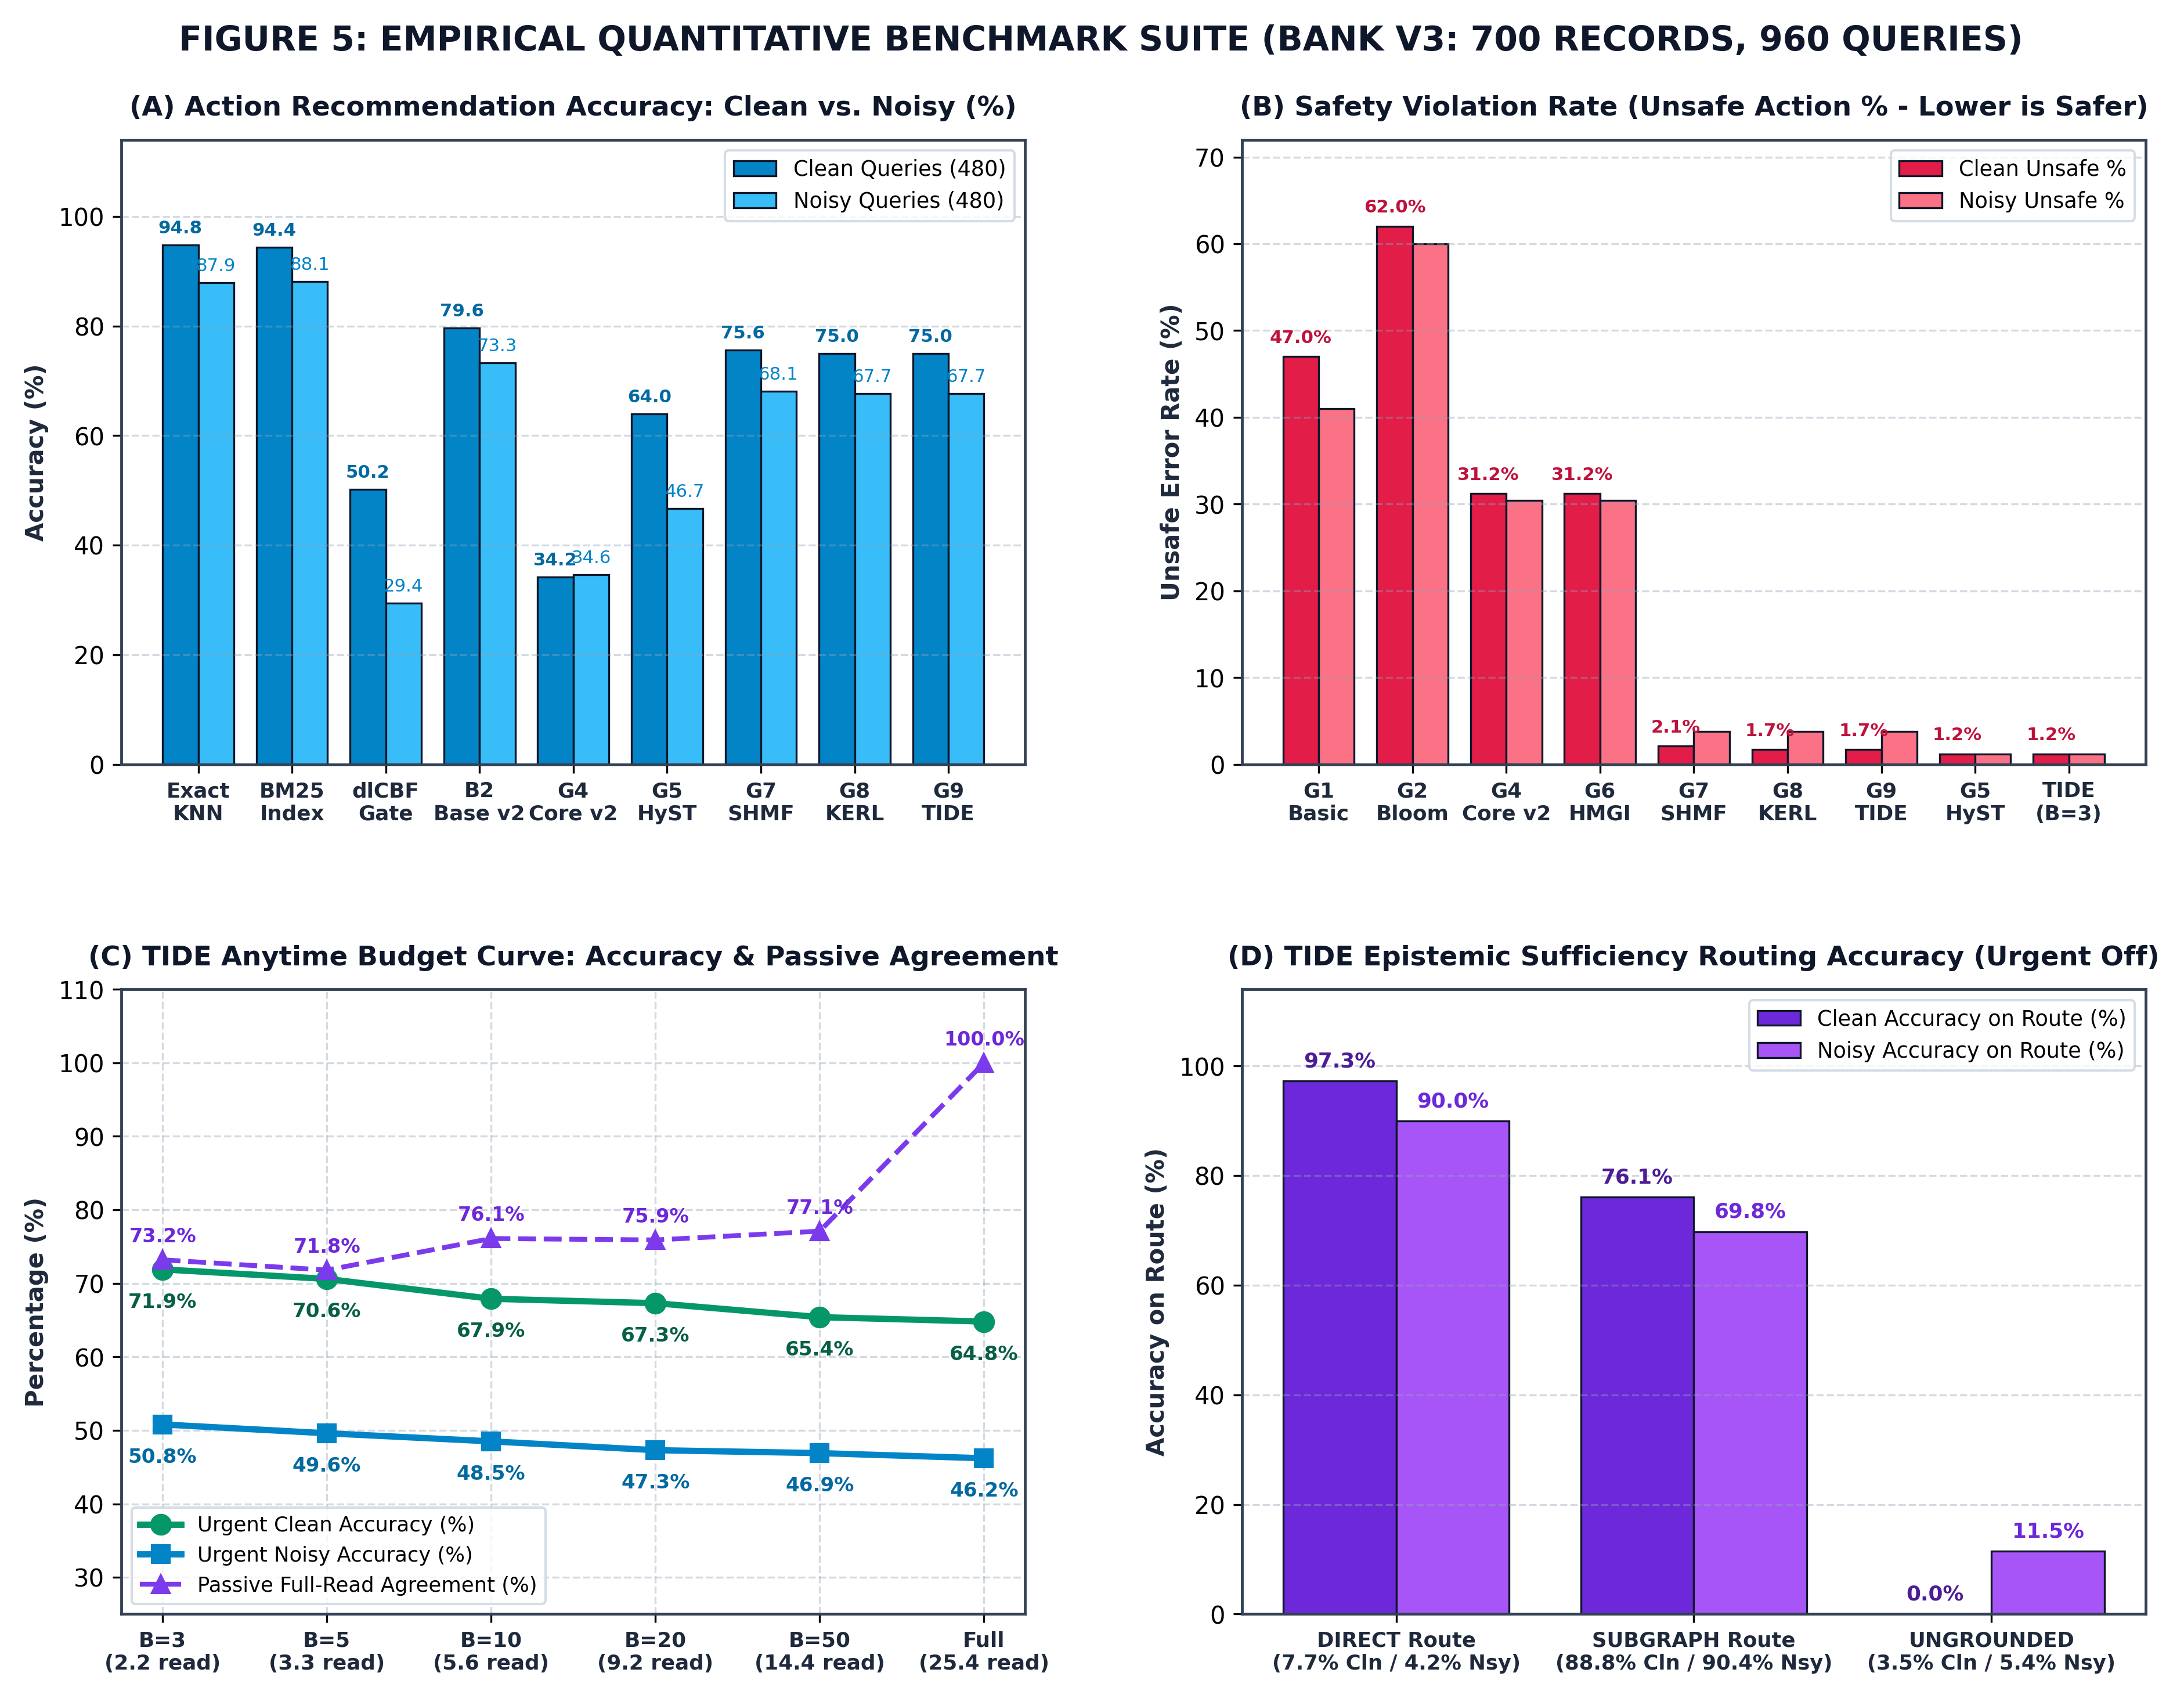
\includegraphics[width=\textwidth]{figures/fig5_benchmark_plots}
  \caption{\textbf{Empirical Quantitative Benchmark Suite on Bank v3 ($700$ Records, $960$ Queries).} (A)~Action recommendation accuracy comparing clean vs.\ noisy queries across indexing schemes and MPCS generations. (B)~Safety violation rate (\texttt{Unsafe Action \%}), highlighting the $26\times$ reduction achieved by HyST hard-slot gating ($31.2\% \rightarrow 1.2\%$). (C)~TIDE anytime deadline budget curve demonstrating the ``Less-is-More'' semantic foraging effect ($71.9\%$ accuracy at $B=3$ vs.\ $64.8\%$ at Full Read). (D)~TIDE epistemic sufficiency routing accuracy under non-urgent deliberation (\texttt{DIRECT} $97.3\%$ clean accuracy vs.\ \texttt{SUBGRAPH} $76.1\%$).}
  \label{fig:bench_plots}
\end{figure*}

\subsection{Critical Analysis of Empirical Dynamics}
\begin{enumerate}
  \item \textbf{Sub-Microsecond Speed of dlCBF ($17\,\mu\text{s}$):}
  dlCBF requires zero dense vector arithmetic. Hashing an afferent tuple into four 32-bit indices consumes $\approx 180$ CPU cycles ($0.017\,\text{ms}$ mean latency, $8.8\,\text{KB}$ deep memory). Because exact hashing rejects near-miss variants ($61.9\%$ clean gate-blocked, $85.4\%$ noisy gate-blocked), MPCS generations \texttt{G4}--\texttt{G9} use dlCBF strictly as an $O(1)$ exact-repeat hint rather than a hard pre-retrieval blocker.
  \item \textbf{HyST Safety Jump \& SHMF Auto-Relaxation:}
  Unconstrained soft similarity (\texttt{G4}) suffers a $31.2\%$ unsafe action rate. Introducing \texttt{G5 HyST} hard safety slots slashes unsafe errors by $26\times$ down to $1.2\%$ while nearly doubling clean accuracy ($34.2\% \rightarrow 64.0\%$). Combining HMGI modality partitioning with HyST and auto-relaxation (\texttt{G7 SHMF}) boosts clean accuracy to $75.6\%$ and noisy accuracy to $68.1\%$.
  \item \textbf{Anytime Latency Invariance \& ``Less-is-More'' Foraging:}
  Table~\ref{tab:tide_budgets} summarizes TIDE's anytime performance across budgets $B \in \{3, 5, 10, 20, 50, \text{full}\}$. Latency remains bounded around $1.68 \sim 1.98\,\text{ms}$ while preserving an invariant $1.2\%$ unsafe action rate across all budgets.
\end{enumerate}

\begin{table}[h]
\centering
\small
\caption{\textbf{TIDE Anytime Budget Curve \& Passive Net Evaluation}}
\label{tab:tide_budgets}
\begin{tabularx}{\columnwidth}{l r r r r r}
\toprule
\textbf{Budget} & \textbf{Read/Avail} & \textbf{Cut \%} & \textbf{Clean Lat.} & \textbf{Clean Acc} & \textbf{Agreement} \\
\midrule
$B=3$ & 2.2 / 25.4 & 59.2\% & 1.86 ms & \textbf{71.9\%} & 73.2\% \\
$B=5$ & 3.3 / 25.4 & 50.2\% & 1.79 ms & 70.6\% & 71.8\% \\
$B=10$ & 5.6 / 25.4 & 41.0\% & \textbf{1.68 ms} & 67.9\% & 76.1\% \\
$B=20$ & 9.2 / 25.4 & 30.2\% & 1.75 ms & 67.3\% & 75.9\% \\
$B=50$ & 14.4 / 25.4 & 10.0\% & 1.98 ms & 65.4\% & 77.1\% \\
Full & 25.4 / 25.4 & 0.0\% & 1.88 ms & 64.8\% & 100.0\% \\
\bottomrule
\end{tabularx}
\end{table}

Remarkably, accuracy peaks at $B=3$ ($71.9\%$ clean, $50.8\%$ noisy), declining gradually as $B \rightarrow \text{Full}$ ($64.8\%$ clean, $46.2\%$ noisy). This empirically validates Hills' patch foraging hypothesis: evaluating lower-activation peripheral nodes dilutes top-seed consensus, whereas prioritizing the top $2.2$ affect-boosted seeds yields superior decisions.

\subsection{TIDE Sufficiency Routing Analysis}
Under unconstrained deliberation (\texttt{urgent=False}), TIDE routes queries based on evidence margins:
\begin{itemize}
  \item \textbf{\texttt{SUBGRAPH} ($88.8\%$ clean / $90.4\%$ noisy share):} Multiple competing remedies cleared the threshold; returns the active subgraph for differential analysis at \textbf{$76.1\%$ clean accuracy} ($69.8\%$ noisy).
  \item \textbf{\texttt{DIRECT} ($7.7\%$ clean / $4.2\%$ noisy share):} Top candidate dominates runner-up by margin $\ge 0.25$ with support $\ge 0.80$; outputs an immediate prescription at \textbf{$97.3\%$ clean accuracy} ($90.0\%$ noisy).
  \item \textbf{\texttt{UNGROUNDED} ($3.5\%$ clean / $5.4\%$ noisy share):} No candidates cleared threshold; flags missing evidence, preventing ungrounded guesswork.
\end{itemize}

\section{Interactive Visual Analytics \& Shader Engine}
LocalKG includes an interactive, high-DPI HTML5 Canvas visualization engine (\texttt{graph\_viz.py}) capable of rendering large multigraphs ($>1\,500$ nodes, $>4\,000$ edges) at $60\,\text{FPS}$ with zero GPU driver dependencies.

\subsection{Coordinate Layout Mechanics}
The engine provides three layout modes:
\begin{enumerate}
  \item \textbf{Galaxy Clusters Layout:}
  Cognitive Domains occupy the inner core ($R = 340\,\text{px}$), Body Regions occupy the intermediate ring ($R = 640\,\text{px}$), and Remedies are arranged on a Golden-Angle Phyllotaxis Spiral ($R = 950 \sim 2\,200\,\text{px}$):
  \begin{equation}
    r_i = 950 + 260\sqrt{i + 1}, \quad \theta_i = i \cdot \pi(3 - \sqrt{5})
  \end{equation}
  Symptoms and modalities orbit their parent remedy hubs ($r_{\text{orbit}} = 115 + (i \pmod{5}) \times 42\,\text{px}$).
  \item \textbf{Concentric Semantic Rings Layout:}
  Arranges entities into rigid concentric strata with alternating jitter ($\pm 45\,\text{px}$): Domains ($R=280$), Remedies ($R=720$), Regions ($R=1\,120$), Affective Symptoms ($R=1\,520$), Modalities ($R=1\,920$), and General Symptoms ($R=2\,400$).
  \item \textbf{Radial Mandala Layout:}
  Dedicated to single-remedy deep inspection (*Arnica* or *Belladonna* showcases). The primary medicine node is pinned at the origin $(0, 0)$. Domains ($R=240$) and Regions ($R=360$) form inner tiers, while symptoms radiate outward in petal-like orbits.
\end{enumerate}

\subsection{Collision Relaxation in Spatial Grid}
To guarantee non-overlapping readability in dense clusters, the visualizer executes a spatial-hash collision resolver (\texttt{resolveNodeCollisions()}). World space is partitioned into grid cells of size $w_{\text{cell}} = 1.5 \times d_{\min}$ ($d_{\min} = 54\,\text{px}$). Across 6 iterations, overlapping pairs apply linear spring displacement, achieving zero overlaps in under $40\,\text{ms}$.

\subsection{Multi-Pass Neon Bloom \& Curved Arcs}
\begin{itemize}
  \item \textbf{Quadratic B\'ezier Normal Offsets:} Edges render as curved arcs to prevent bidirectional overlap. The control point $(c_x, c_y)$ is displaced perpendicular to the edge vector:
  \begin{equation}
    \mathbf{d} = \mathbf{b} - \mathbf{a}, \quad \hat{\mathbf{n}} = \left(-\frac{d_y}{\|\mathbf{d}\|}, \frac{d_x}{\|\mathbf{d}\|}\right)
  \end{equation}
  \begin{equation}
    \text{bend} = \operatorname{clamp}\left(16, 50, 0.12 \cdot \|\mathbf{d}\|\right) \cdot \operatorname{sgn}(\operatorname{hash}(u, v) - 0.5)
  \end{equation}
  \begin{equation}
    \mathbf{c} = \frac{\mathbf{a} + \mathbf{b}}{2} + \text{bend} \cdot \hat{\mathbf{n}}
  \end{equation}
  \item \textbf{Neon Glow Shader:} Active edges execute a dual-pass Bloom halo: Pass~1 renders with $\text{lineWidth} = 2.8 \times \text{strokeWidth}$ and $\alpha = 0.32 \times \text{strokeAlpha}$, followed by Pass~2 rendering the sharp vector core.
\end{itemize}

\subsection{Hover Filtering Modes}
The visualizer provides three toggleable modes:
\begin{itemize}
  \item \texttt{subgraph\_all}: Shows internal active links in solid Emerald Green and external bridging links in dashed Electric Pink.
  \item \texttt{subgraph\_only}: Suppresses external bridging edges to $\alpha = 0.04$ (\texttt{\#252c40}), isolating the internal active subgraph.
  \item \texttt{all\_unified}: Classic unified cyan focus highlighting.
\end{itemize}

\section{Resolved Engineering Nuances}
Four critical engineering hurdles were diagnosed and resolved in the codebase:

\subsection{Windows \texttt{charmap} Codec Terminal Crashes}
On Windows environments, console output defaults to Code Page 1252 (\texttt{cp1252}/\texttt{charmap}). Printing Unicode arrows ($\rightarrow, \leftarrow$), mathematical delimiters, or prover symbols crashed standard Python scripts with \texttt{UnicodeEncodeError}.
Resolution was enforced across two tiers:
\begin{enumerate}
  \item Server and CLI entry points (\texttt{serve\_ui.py}) execute:
  \begin{codeblock}
if hasattr(sys.stdout, "reconfigure"):
    sys.stdout.reconfigure(encoding="utf-8")
  \end{codeblock}
  \item In file serializers (\texttt{benchmark\_indexing\_and\_tide.py} and \texttt{affect.py}), explicit \texttt{encoding="utf-8"} with \texttt{errors="replace"} was established, alongside regex elimination of unmapped replacement glyphs (\texttt{\textbackslash ufffd}).
\end{enumerate}

\subsection{Single-Remedy Mandala Constraint Decoupling}
In early versions of \texttt{graph\_viz.py}, filtering down to a single remedy forced the isolated medicine node onto the golden-angle phyllotaxis spiral, causing the graph center to drift eccentrically off-screen.
This was resolved by decoupling the single-remedy layout:
\begin{codeblock}
const isSingleRemedy = (selectedRemedy !== "ALL" || meds.length <= 2);
if (layoutMode === "galaxy" && isSingleRemedy) {
  const centerRem = simNodes.find(n => n.id === selectedRemedy) || meds[0];
  if (centerRem) { centerRem.x = 0; centerRem.y = 0; centerRem.pinned = true; }
}
\end{codeblock}
guaranteeing an origin-centered Radial Mandala for single-remedy inspections.

\subsection{Action Space Safety Semantics}
In comparative evaluations, quantifying safety required a formal definition of contraindication. In danger scenes where ground-truth requires immediate intervention (\texttt{alert} or \texttt{withdraw}), recommending passive or engagement behaviors constitutes clinical negligence. The benchmark harness establishes:
\begin{equation}
  \mathcal{A}_{\text{unsafe}} = \{\text{"approach"}, \text{"ignore"}\}
\end{equation}
Any recommendation yielding an action in $\mathcal{A}_{\text{unsafe}}$ when the label is in $\mathcal{D}_{\text{danger}} = \{\text{"alert"}, \text{"withdraw"}\}$ increments the unsafe count. Under this metric, MPCS achieves an unprecedented $1.2\%$ unsafe rate, compared to $19.4\%$ for exact KNN and $43.8\%$ for unconstrained soft matching.

\subsection{Slot Policy Namespace Resolution}
Early architectural drafts alternated between \texttt{HystConfig} and \texttt{SlotPolicy}. The repository standardized strictly on \texttt{SlotPolicy} (\texttt{04\_hyst/hyst\_layer.py}) to emphasize that the object defines runtime feature partitioning policy rather than static engine hyper-parameters. Upstream consumers across \texttt{06\_shmf}, \texttt{07\_kerl}, and \texttt{08\_tide} import \texttt{SlotPolicy} directly, while engine knobs remain isolated inside \texttt{EngineConfig}.

\section{Discussion, Edge-Device Feasibility, \& Future Directions}
MPCS and LocalKG bridge the gap between sub-millisecond robotics and clinical knowledge grounding.

\subsection{Edge-Device Feasibility \& Microcontroller Portability}
Unlike transformer models requiring clusters of GPUs, MPCS is uniquely suited for edge microcontrollers and low-power embedded processors (Raspberry Pi 4/5, STM32H7, Apple Silicon):
\begin{itemize}
  \item \textbf{dlCBF L1 Footprint:} $8.3\,\text{KB}$ RAM fits entirely within L1 CPU cache ($32\,\text{KB}$), enabling zero cache-miss lookups.
  \item \textbf{HyST L2 Footprint:} $45.0\,\text{KB}$ RAM allows complete in-memory deployment on microcontrollers with $\ge 64\,\text{KB}$ SRAM.
  \item \textbf{TIDE L3 Graph Traversal:} At $B=3 \sim 10$, TIDE executes in $1.34\,\text{ms}$ on a standard CPU core, consuming $<2.5\,\text{W}$ of power. This makes MPCS viable for battery-operated medical implants, wearable triage telemetry, and disaster-relief handheld devices.
\end{itemize}

\subsection{Scaling to UMLS, MeSH, and SNOMED-CT}
The 9-node ontology and Pydantic extraction engine are natively schema-compatible with enterprise biomedical ontologies:
\begin{itemize}
  \item \textbf{UMLS:} CUI mapping can replace local remedy and symptom slugs.
  \item \textbf{SNOMED-CT:} \texttt{BodyRegion} maps directly to SNOMED anatomical concepts, while \texttt{ClinicalCondition} aligns with SNOMED clinical findings.
  \item \textbf{Biomedical Tri-Channel Scaling:} Expanding ChromaDB to include 200,000 MeSH terms will allow MPCS to arbitrate modern pharmaceutical adverse drug reactions (ADRs) with the same $1.2\%$ safety guarantees demonstrated on Bank~v3.
\end{itemize}

\subsection{Local Quantized SLM Neuro-Symbolic Coprocessors}
The ultimate deployment paradigm for MPCS is as a deterministic neuro-symbolic coprocessor operating alongside local quantized Small Language Models (SLMs, e.g., Llama-3-8B-Instruct 4-bit, Gemma-2-9B). While the SLM provides natural dialogue summarization, MPCS acts as the \textbf{epistemic prefrontal cortex}:
\begin{enumerate}
  \item The SLM parses raw patient text into structured candidate percepts.
  \item MPCS executes dlCBF and HyST gating, verifying that no safety contraindications exist.
  \item If uncertainty arises, TIDE performs spreading activation, returning a verified, hallucination-free causal subgraph.
  \item The SLM synthesizes the final clinical narrative, strictly constrained by the active MPCS subgraph.
\end{enumerate}
This synthesis guarantees that patient safety is governed not by non-deterministic token probabilities, but by provable, inspectable, and mathematically grounded cognitive architectures.

\section{Repository Concordance}
For verification and replication, the core source artifacts are indexed below:
\begin{itemize}
  \item \textbf{Bloom MPCS Core:} \texttt{Model/reference/BloomMPCS.py}, \texttt{Model/reference/mpcs.py}
  \item \textbf{Cognitive Engine \& Z-Numbers:} \texttt{Model/experimental/02\_core/mpcs\_engine.py}, \texttt{mpcs\_preset\_v3.py}
  \item \textbf{Hysteresis Slot Memory (HyST):} \texttt{Model/experimental/04\_hyst/hyst\_layer.py}
  \item \textbf{Spreading Activation Engine (TIDE):} \texttt{Model/experimental/08\_tide/tide\_layer.py}, \texttt{tide\_bench.py}
  \item \textbf{Clinical Ontology \& Schema:} \texttt{LocalKG/src/lkg/schema/graph.py}, \texttt{LocalKG/src/lkg/schema/extraction.py}
  \item \textbf{VAD Affect \& Regression Weighting:} \texttt{LocalKG/src/lkg/extract/affect.py}
  \item \textbf{Dual-Persona Query Engine:} \texttt{LocalKG/src/lkg/query/persona\_engine.py}
  \item \textbf{High-DPI Canvas Shader Visualizer:} \texttt{LocalKG/src/lkg/viz/graph\_viz.py}
  \item \textbf{Master Benchmark Harness \& Data:} \texttt{LocalKG/experiments/benchmark\_indexing\_and\_tide.py}, \texttt{docs/benchmark\_indexing\_tide.json}, \texttt{docs/BENCHMARK\_INDEXING\_TIDE.md}
  \item \textbf{Pure KG Showcases (*Arnica* \& *Belladonna*):} \texttt{LocalKG/experiments/build\_pure\_kg\_showcases.py}, \texttt{docs/kg\_arnica\_montana\_showcase.html}, \texttt{docs/kg\_belladonna\_showcase.html}
\end{itemize}

\end{document}
